\chapter{Introduction}
\label{chapter:introduction}
\textit{"An approximate answer to the right problem is worth a good deal more than an exact answer to an approximate problem"}- John Tukey

\section{Chapter Overview}
Decision support systems~(DSS) are information system that support business or organizational decision-making activities~\cite{hackathorn1981organizational}. A typical DSS takes a set of input and analyzes them to generate actionable insights from which DSS `decisions' are generated. Subsequently, the decision is annotated or validated with user knowledge and expertise. In other words, a DSS is often a computerized program, which analyse massive amounts of data to assists in decision-making. On the other hand, a DSS that can perform selected cognitive decision-making functions based on artificial intelligence~(AI) or intelligent agents technologies called intelligent DSS. 

\hspace*{3.5mm} Due to recent advancement and performance across domains like computer vision, natural language processing, multimedia analytics, and business analytics, an AI-guided DSS could eventually be applied to various automated decision-making processes. In an AI-guided or intelligent DSS, a set of learning algorithms are embedded that perform cognitive decision-making. These learning algorithms mostly include various machine learning~(ML) algorithms that acts one of the most common forms of AI. 
ML is about using a set of statistical and mathematical algorithms to perform tasks such as concept learning, predictive modeling, clustering, and mining useful patterns can be performed. The most complex forms of ML involve deep learning~(DL), or deep neural network~(DNN) models with many levels of features or variables that predict outcomes that help take meaningful decision. However, DNN models are perceived mostly as `black box' methods because of their not well-understood internal functioning. Besides, they cannot reason their underlying decisions, leaving them incapable of aiding transparent and trustworthy decisions. Consequently, we call such DSS a `black box' model. 

\hspace*{3.5mm} Throughout this thesis we aim to improve the transparency and explainability of such black-box DSSs. This chapter provides a general introduction to this dissertation, provides the motivation for this research, list down the hypotheses and research questions, and outlines the structure of this thesis. 
%In particular, \cref{chapter:preli} discusses the reason of cancer and outlines it's severity.
\Cref{motivations}, outlines the motivation underpinning the DSS based on.  \Cref{problem_challenges}, discusses the research problems and points out several challenges concerning the research problems. \Cref{goals} discusses the goal of this thesis including a workflow diagram. \Cref{hypotheses} presents the hypotheses and research questions derived from the previously reported work on cancer prediction and diagnosis. \Cref{contributions} lists the contributions of this dissertations. \Cref{structure} outlines the organisation and structure of the thesis.

%\section{Introduction}

\section{Motivation}\label{motivations}
Intelligent DSSs are often ML or DL-based DSS, where a ML or DL algorithm is employed to improve the learning experience such that it becomes automatic by reducing the level of human interaction as much as possible. In many domains, applying ML and getting higher prediction accuracy is not enough. Eventhough some ML models maybe better at predicting, detecting, and processing patterns better than humans, they cannot reason or explain. In fact, in many cases, the goal is not only predicting something with a high-level of confidence, rather better understanding. Moreover, real-life data contain heterogeneity, high variability, and high dimensionality, which imposes significant challenges to existing ML methods stimulating the development of DL-based DSS. Nevertheless, our real world experience is multimodal~\cite{mmsurvey}, e.g., while watching a movie, we not only observe the movie itself but the acting, background music, action, background scenario, and landscapes, etc. 

\hspace*{3.5mm} To tackle these, approaches based on DL work better with such high dimensional data, recent studies focused on using different DNN architectures based on autoencoders, convolutional neural network~(CNN), and recurrent neural network~(RNN). Although many existing approaches based on DNN have shown tremendous success in solving such problems, DNN models are perceived mostly as `black box' methods because of their not well-understood internal functioning. Subsequently, they cannot reason their underlying decisions, leaving them incapable of providing transparent and trustworthy decisions. 
Furthermore, since the opaqueness raises numerous legal, ethical, and practical concerns, transparency and accountability in AI-based systems have to ensure. From practical point of view, if we cannot see how the predictions were made, we cannot know what impact will happen on human lives, as the day when such AI-guided machines take life decisions for humans is not very far ahead. To show the impacts of `black-box' DSS, let's see two case studies. 

\subsection{Impacts of `black-box' DSS in financial sector}
The financial sector was one of the first to start experimenting with ML applications for a variety of use-cases. In recent years, financial institutions such as banks and other lenders~(e.g., a bank) are looking to ML as a way to win market share and stay competitive in a changing landscape, and automating many things to handle all of their banking needs. Besides, banks face several unique difficulties when it comes to implementing ML, particularly with regards to ML-based credit models. Even many are not fully aware of the challenges that come with adopting ML in finance. To understand the negative impacts of a `black-box'-based DSS in finance and explain how a lack of transparency may cause problems for banks and consumers that interact with ML-based credit models.

\vspace{-4mm}
\begin{figure*}[h]
	\centering
	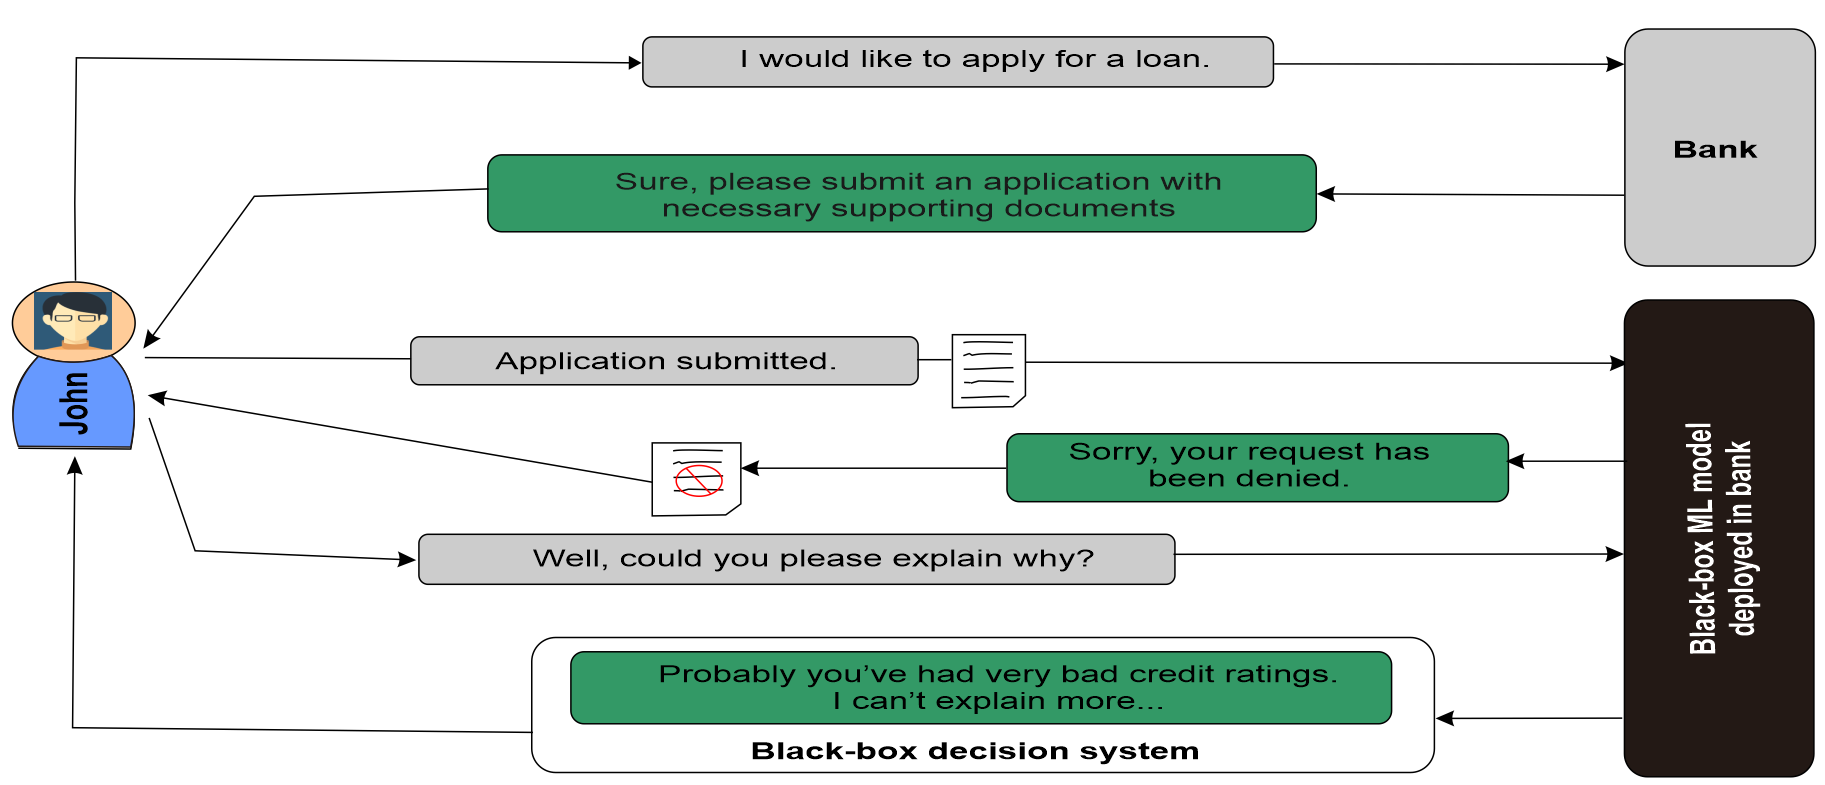
\includegraphics[width=0.9\linewidth,height=80mm]{images/loan.png}
	\caption{Problems of model opacity}
    \label{fig:model_bbm}
    \vspace{-4mm}
\end{figure*}

\hspace*{3.5mm} Let's assume a simple example of a man named John, who is a typical bank customer. Suppose John~(like most customers today) applies for a credit~(loan) from a bank. However, suppose his application got somehow rejected. When he asked the lender why it was the case, they should be able to explain the reason, i.e., in credit underwriting, the bank must be able to explain to applicants why they were rejected. Traditional linear models make this relatively simple as one can easily interpret how the model and the underwriter came to the borrower decision, and they factor in significantly fewer variables than a ML model could. There may be hundreds of variables involved in a ML-based credit model, where the interactions among each of those variables can be variables too. Without rigorous explainability, banks are not able to provide applicants with an adverse action notice that details why they were rejected, information they can use to improve their credit profiles and successfully obtain credit in the future. 

\subsection{Impacts of `black-box' DSS in healthcare}
A more concrete example of using AI-guided systems in healthcare is carcinogenesis. Cancer has been characterized as a heterogeneous disease consisting of many different types and subtypes, making it is one of the deadliest diseases. However, diagnosis and prognosis, especially for specific cancer types is not straightforward. In fact, the diagnosis of a breast cancer patient depends on several distinct molecular subtypes, e.g., multiple factors are involved~(e.g., in cancer diagnosis, estrogen receptor, progesterone receptor, and human epidermal growth factor receptor, providing AI-based diagnoses might not be accurate solely based on CNVs. 

\begin{figure*}[h]
	\centering
	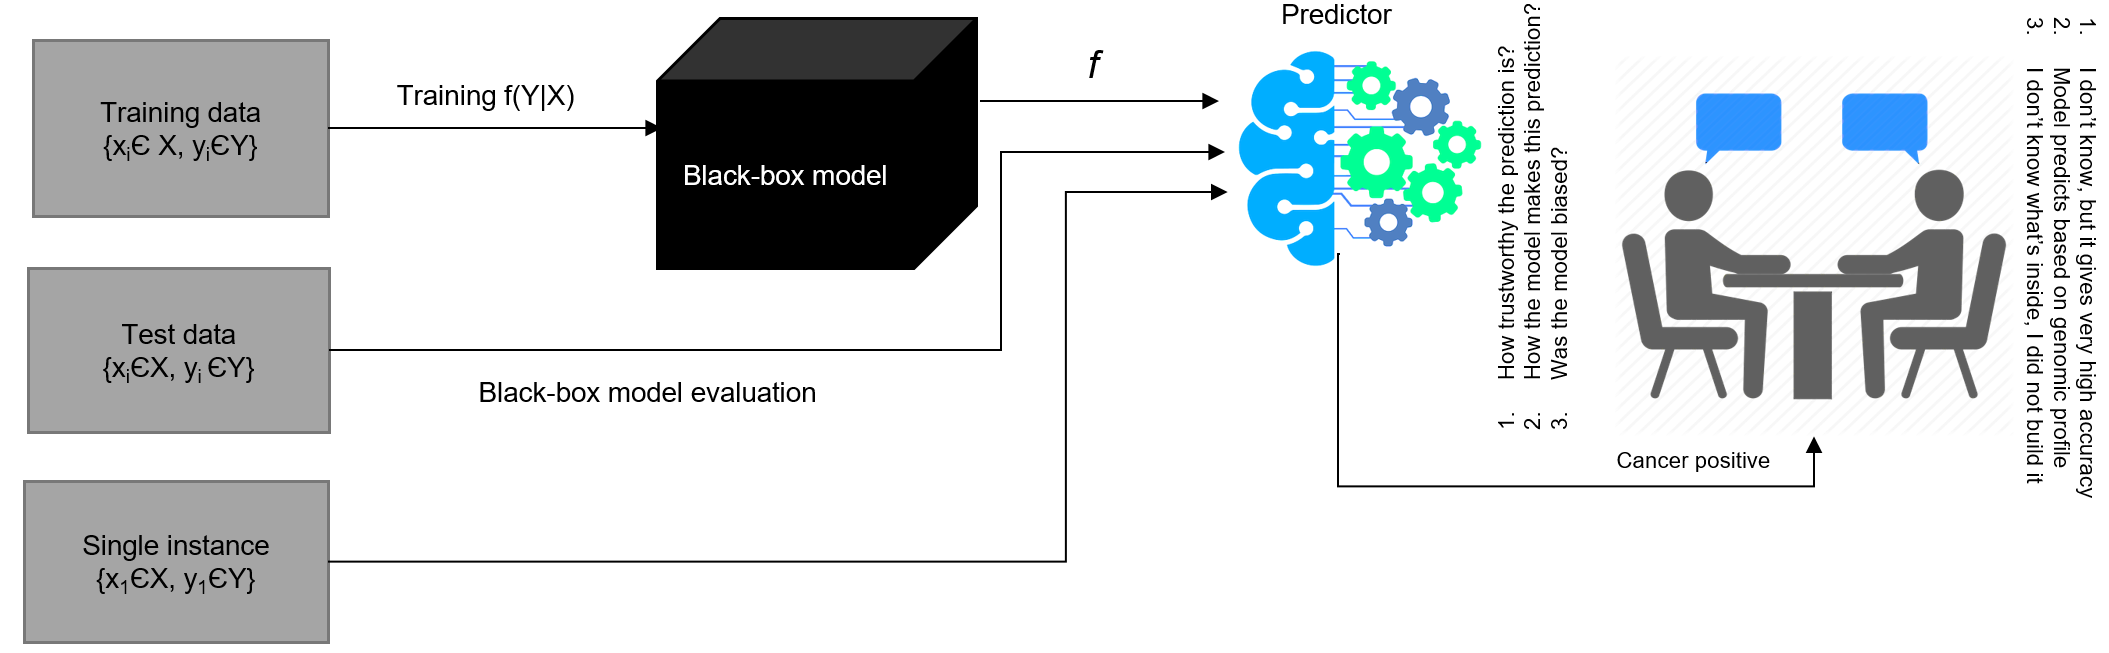
\includegraphics[width=\linewidth,height=60mm]{images/bbm.png}
	\caption{Problems of model opacity}
    \label{fig:model_bbm}
    \vspace{-2mm}
\end{figure*}

\hspace*{3.5mm} This requires using multimodal features based on DNA methylation, gene expression, miRNA expression, and CNVs data by creating a multiplatform network to support each data type, where the DSS based on genomics data from different cohorts will be more reliable. Subsequently, an early diagnosis of cancer~(e.g., classifying cancer patients into high or low risk groups) have become essential in cancer research, as it can facilitate the subsequent clinical management of patients~\cite{kourou2015machine}.  

\subsection{Legal aspects}
Unexplainable ML-based credit models can have serious legal consequences for lenders that use them. The legal landscape is complex and fast-moving across countries, such as the Equal Credit Opportunity Act and Fair Credit Reporting Act~\cite{act2009fair}. In particular, section 609(f)(1) of the Fair Credit Reporting Act %Nevertheless, failure to do so accurately can result in large fines and/or a suspension of banking license. %Noncompliance is perhaps the most vital reason that lenders have been cautious to adopt machine learning for credit scoring and underwriting.
requires that consumers be provided ``all of the key factors that adversely affected the credit score of the consumer in the model used, the total number of which shall not exceed 4". This enforces lenders to be able to explain the models they use to approve and deny credit applicants. 

\hspace*{3.5mm} There are important legality concerns such as The General Data Protection Regulation~(GDPR)~\cite{kaminski2019right} by the European Parliament suggests that individuals should be able to obtain explanations of the decisions made from their data by automated processing, and to challenge the decision. Article 22 states that individuals ``have the right not to be subject to a decision based solely on automated processing" and ``whenever human subjects have their lives significantly impacted by an automatic decision-making machine, the human subject has the right to know why the decision is made", i.e., `right to explanation'. 
%In other words, 

\hspace*{3.5mm} In summary, GDPR prohibits the use of ML for automated decisions unless a clear explanation of the logic used to make each decision is well explained. Another such AI-guided clinical decision support system~(CDSS) is used in healthcare is increasingly been applied and adopted. For example, AI-based systems have already been deployed in diagnosis, treatment recommendations, patient engagement, and administrative activities. There are many instances, where AI already outperforming healthcare tasks in automated diagnoses and treatment in clinical setting, e.g., outperforming radiologists at spotting malignant tumours, model the progression and treatment of cancerous conditions. Besides, AI is guiding researchers in how to construct cohorts for costly clinical trials~\cite{davenport2019potential}. 

%\subsection{Issues with existing interpretable models}
%we don't fully understand how and which factors tend a model to make a prediction right and why it will fail in certain cases
%\Cref{fig:chapter_2_wf} outlines the workflow of the proposed approach to make the model explainable. 

\section{Thesis Goal} \label{thesis_goal}
%Although these models have shown tremendous success in exhibiting high confidence, they are mostly perceived as `black box' methods because of a lack of understanding of their internal functioning. 
Although, not every prediction made by an ML algorithm needs an explanation~\cite{stiglic2020interpretability}, in many cases, ML models itself have to be interpretable enough to ensure that the decisions made by the system is not only accurate, but also trustworthy~\cite{mehrabi2019survey}. 
Coming back to our cancer diagnosis case study. Current cancer typing methods focused on employing ML approaches and using mixed data types to handle the high dimensionality and heterogeneity. However, since predicting cancer types and providing explanation are two of our desired objectives, someone might ask why don't we simply use interpretable models? 
%Eventhough, they perform well, but lack the capability of explain the diagnoses decisions. 
It is well-known that interpretable models and their inner working mechanism are simple. However, such a simple model lacks the capacity and flexibility to capture complex relations and interactions between high dimensional genomic data. In principle, except for the linear and tree-based models, DNN models are perceived mostly as `black box'. Hence often we don't fully understand how and which factors tend the model itself to reach a diagnosis decision, e.g., prediction. % right and why it will fail in certain cases methods as w of their not well-understood internal functioning. Often, . These are serious drawbacks.

\begin{figure*}[h]
	\centering
		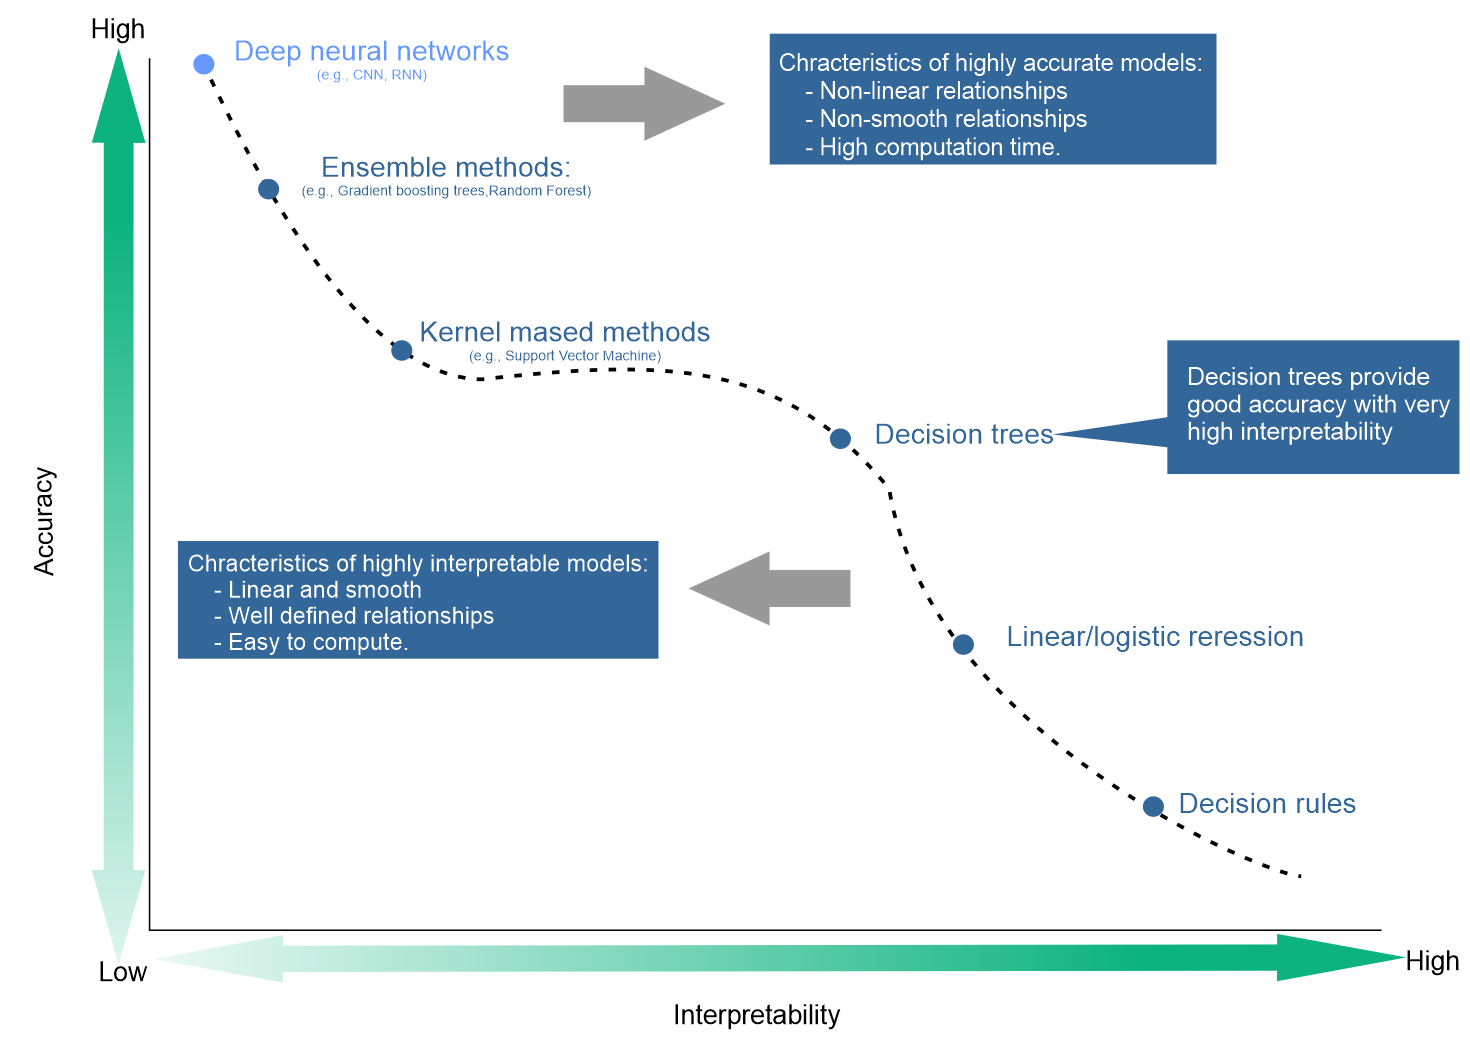
\includegraphics[width=0.8\linewidth,height=80mm]{images/acc_vs_xai.png}
		\caption{Accuracy vs. interpretability trade-off}
        \label{fig:acc_vs_xai}
\end{figure*}

%Higher interpretability of an ML model means easier comprehension and explanation of future predictions for end-users. 
\hspace*{3.5mm} This evolves a fundamental trade-off between accuracy and interpretability: the more interpretable a model is, the less accurate it is. In other words, the most accurate ML models are the least interpretable, as shown in \cref{fig:acc_vs_xai}. Knowing the cancer type and identifying most relevant biomarkers are the prerequisites for an oncologist to recommend more accurate treatments and drug repositioning. The latter only can be achieved with meaningful explanations, which helps healthcare experts to make reasonable and data-driven decisions to provide personalized diagnosis or treatment decisions that can lead to higher quality of service in healthcare~\cite{stiglic2020interpretability}. To the end, developing an explainable DSS to improve the transparency and trustworthiness for cancer diagnosis is the main goal of this thesis, such that the DSS: i) able to generate accurate and trustworthy predictions in a transparent way, ii) can provide human-interpretable explanations of the decisions made, iii) can identify and explain misclassified instances, iv) can validate the decisions based on domain-knowledge from a knowledge base~(KB), v) can produce and help disseminate new knowledge. Based on accurate predictions and human-interpretable explanations, we can identify cancer types and learn similarities between cancer patients. This will help the doctors to answer why, how, and what types of questions asked by the patients. %e what types of decision are made and why. 

\section{Problem Formulation} \label{problem_challenges}
The problem of classifying individuals is grouping them into a specific cancer type based on their genomic profile. Therefore, the cancer typing tasks can be formulated as prediction task in a multi-class classification setting. However, instead of relying on interpretable models, we train several DNN architectures to generate accurate and robust `black-box' models, as shown in \cref{fig:chapter_2_wf}. From a given genomic dataset $D$ about $n$ patients, $X$ = ${\mathbf{\{x_1,x_2,..., x_n}}\}$, we can consider classifying an individual $x_i$ into a specific cancer type based on his or her genomic profile, where $x_k \in \mathbb{R}^{d}$. However, instead of classifying samples directly using their original representation $X$, we first transform the data with a nonlinear mapping $F_{\theta}: X \rightarrow Z$, where $\theta$ are learnable parameters and $Z \in \mathbb{R}^{K}$ is the learned or embedded feature space, where $K \ll D$. 

\begin{figure*}[h]
	\centering
		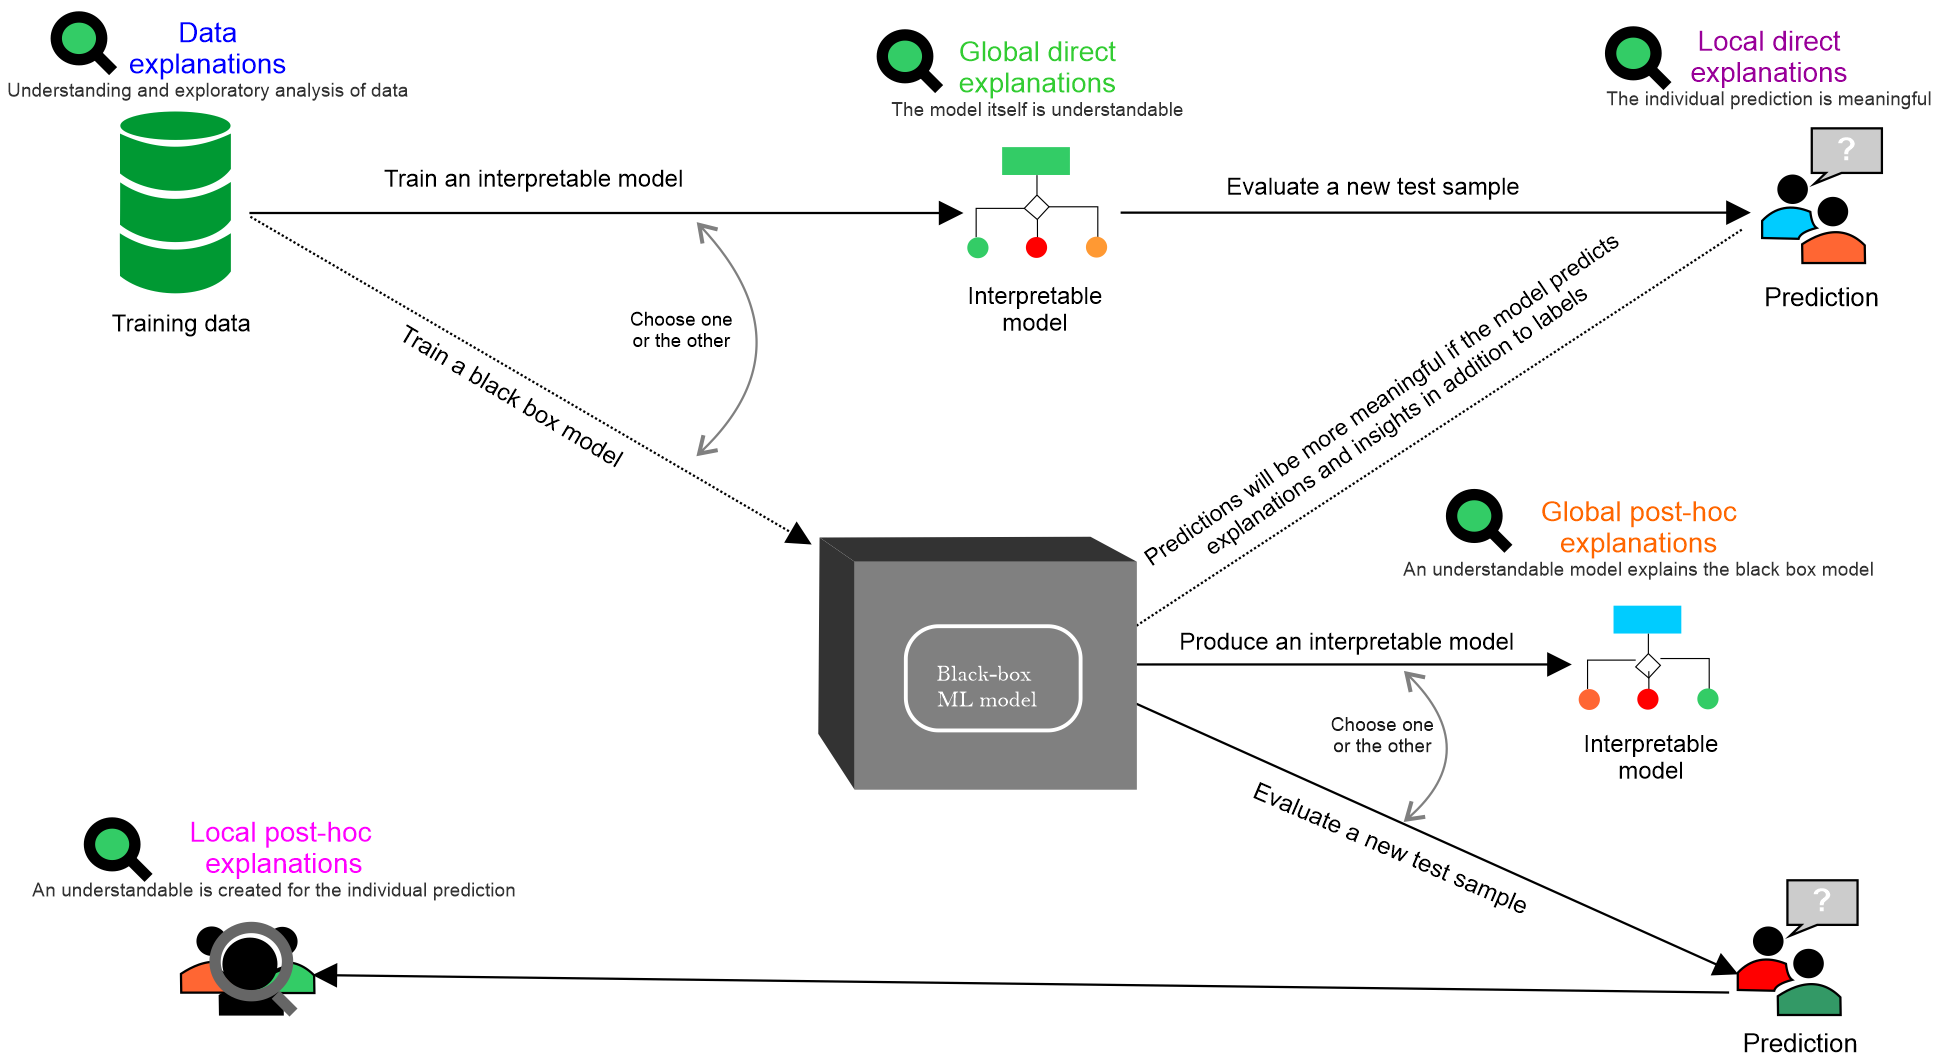
\includegraphics[width=\linewidth,height=100mm]{images/g_t_l_xai.png}
		\caption{Workflow of the proposed approach to make the model explainable}
        \label{fig:chapter_2_wf}
\end{figure*}

\hspace*{3.5mm} To parametrize $F_{\theta}$, we employ neural network-based representation learning~(e.g., autoencoders) due to their function approximation properties and feature learning capabilities~\cite{xie2016unsupervised} from genomic data. Based on the embedding $Z$, classifier $F$ maps an input $x$ to an output $F: \mathbb{R}^{d} \mapsto y$. When we assume $F$ has a parametric form, we write $F_{\theta}$, where ${L}(F(x), y)$ denotes the loss function used to train $F$ on $D$ of input-output pairs $(x,y)$. However, since the decision made by the model cannot be traced back to the inputs, nor is it clear why the outputs are transformed the way they are, we treat $F$ a `black-box' model. 

\hspace*{3.5mm} By embedding both local and global interpretability logic, we make ``black-box" model $F$ interpretable in a post-hoc manner. We explain a data point $x$ using an explanation function $g$. Local interpretability refers to an explanation giving reasoning why the model $F$ has predicted $F(x)$ for a data point $x$, during inferencing. Since providing human-level interpretability by ``zooming in" individual predictions makes the explanation more evident~\cite{ribeiro2018anchors}, we answer the following questions based on local explanation methods: 

\vspace{-2mm}
\begin{itemize}[noitemsep]
    \item Which feature $x \in X$ was most important for a certain prediction with $F$? 
    \item Which training data point $z \in \mathbb{R}^{K}$ was most important to $F(x)$? 
    \item What minimal change is necessary to input $x$ to change the output $F(x)$~(e.g., sensitivity analysis)? 
\end{itemize}
\vspace{-2mm}

\hspace*{3.5mm} Global interpretability signifies the overall transparency of the model inside a model on an abstract level. We answer following questions based on global explanation methods: 

\vspace{-2mm}
\begin{itemize}[noitemsep]
    \item Which features in $X$ were most important across predictions for $F$? 
    \item Which training data points $z \in \mathbb{R}^{K}$ were most important to $F(X)$? 
    \item What minimal change is necessary to input $X$ to change the output $F(X)$~(e.g., sensitivity analysis)? 
\end{itemize}
\vspace{-2mm}

\begin{sidewaysfigure*}
	\centering
	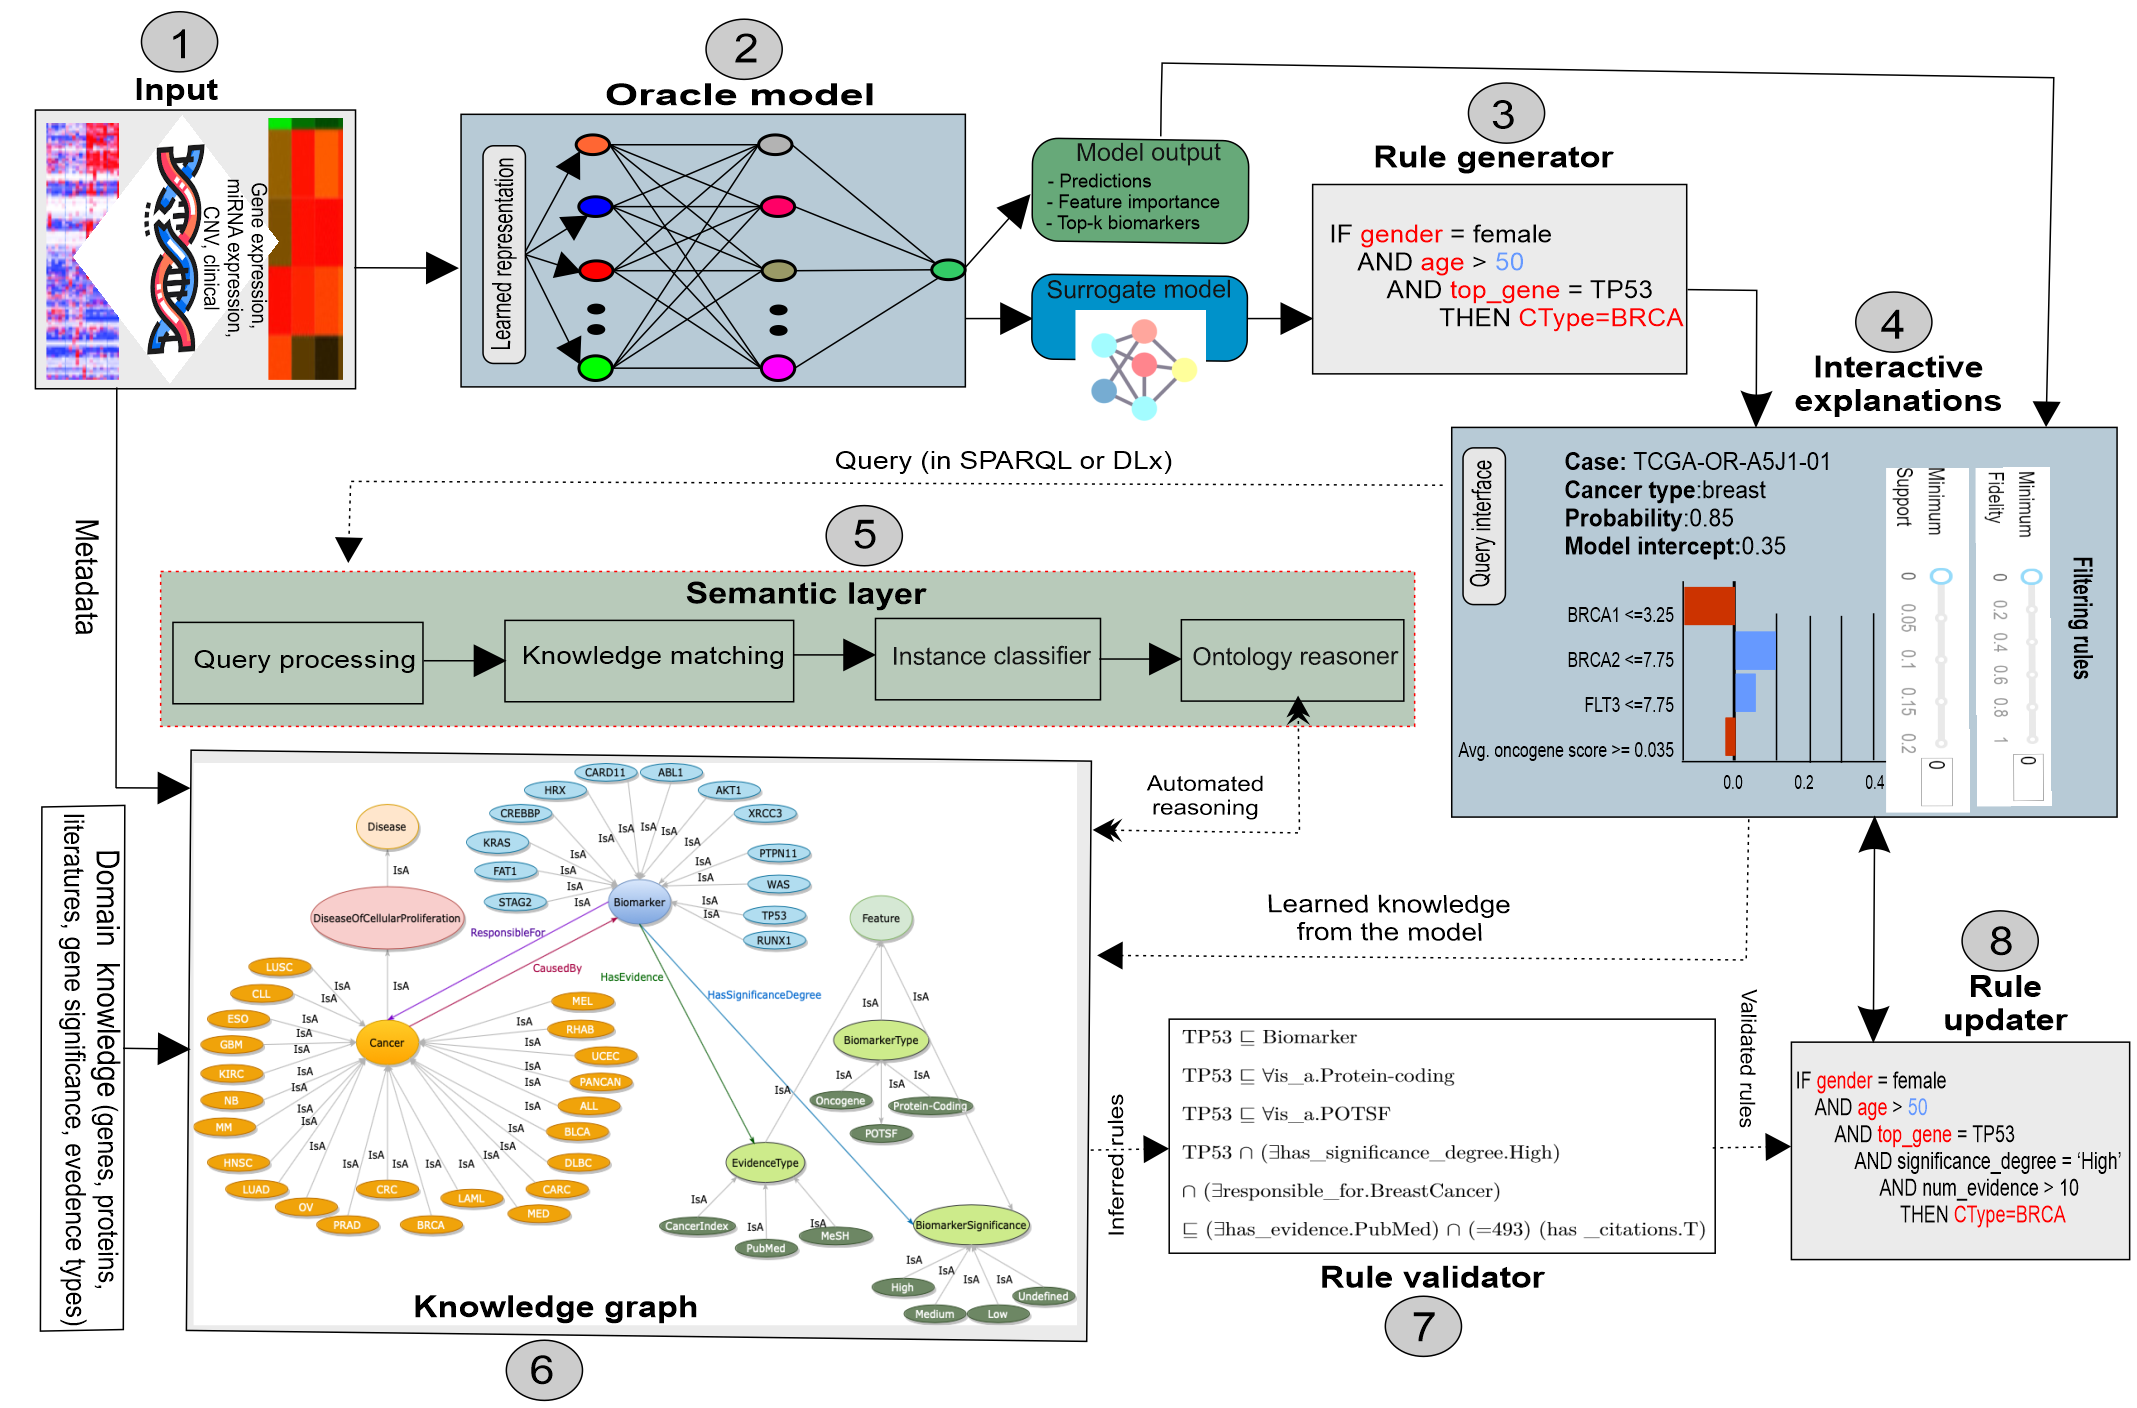
\includegraphics[width=\textwidth]{images/reasoning_wf.png}	
    \caption{Workflow for improving the explainability and transparency of a clinical DSS}
	\label{fig:wf_overall_approach}
\end{sidewaysfigure*}

\hspace*{3.5mm} Further, we validate our findings through functional analysis to make sure the selected genes are biologically trustworthy for the corresponding tumor types. In particular, based on annotations from the TumorPortal, we will validate our findings to ensure biological relevance.  \Cref{fig:wf_overall_approach} depicts the workflow of the proposed approach for making the DSS transparent and explainable for cancer diagnosis.

%\hspace*{3.5mm} In the same line, symbolic reasoning over neural networks~(aka. neuro-symbolic reasoning), which can fuse the ability of DNNs models can be used to learn probabilistic correlations from scratch alongside abstract and higher-order concepts in order to provide human-interpretable explanations, and error corrections. 

%\subsection{Scope of the thesis}
%In the present study, a novel OA quantification solution based on multimodality integration is applied to overcome the limitations of the state-of-the-art approaches by effectively getting rid of the negative influences stemming from modality-forming principles. In terms of their complementary and application range, following a series of preprocessing methods, including contrast enhancement, noise elimination, and multi-slice integration, aiming at the same patient, radiographs and MRIs from axial, sagittal as well as coronal plane are respectively classified by their extracted features in the detected ROIs. Given supplying reliability and objectivity of the grading process, class-discriminating attention maps are generated by Class Activation Maps (CAM), prior to the averaging ensemble of models with the same modality and multimodality. 

\section{Hypotheses and Research Questions} \label{hypotheses}
To disseminating biological knowledge about carcinogenics through the proposed XAI system, the author suggests the following hypotheses to solve several research questions.  

\subsection{Research questions}
To develop an explainable model and to improve the fairness and transparency of a clinical decision support system~(CDSS), this thesis attempts to solve the following research questions: 

\vspace{-2mm}
\begin{itemize}[noitemsep]
    \item \textbf{RQ1}: \textit{How can multimodal data be more effective than unimodal data to provide accurate decision?} As mentioned earlier, multiple factors are involved in cancer diagnosis, genomics data such as GE, miRNA expression, copy numbers, and clinical outcome have to use together to build a more efficient model to accurately predict the outcome of a diagnosis decision.  
    \item \textbf{RQ2}: \textit{How to identify relevant features or factors for a certain decision?} Identification of important biomarkers that contributed most~(i.e., some of the features have a higher impact than others), which facilitates the identification and validation of the presence of cancer and also help determine its stage, subtype, and whether they will respond to therapy. Cancer biomarkers are also of potential therapeutic targets and a key in sequence-specific gene silencing therapy against cancer by selectively silencing aberrantly activated oncogenes.  
    \item \textbf{RQ3}: \textit{How to provide human-understandable interpretations of the decisions using decision rules?} Decision rules are more effective at providing intuitive explanations. Using a set of rules, it is possible to explain a decision directly to humans with the ability to look up the reason for a decision. 
    %\textbf{${RQ}_5$}: How to generate human-interpretable decision rules to provide transparent cancer diagnosis? \\
    \item \textbf{RQ4}: H\textit{ow to disseminate and validate embedded domain knowledge in the model?} An explainable ML model can not only provide predictions, but also insights such as gave top biomarkers, gene correlations, biomarkers types, etc. These help understand the mechanisms of carcinogenesis by further validating the diagnosis with expert and domain knowledge. 
    \item \textbf{RQ5}: \textit{How to score a `black-box' model on transparency?} Knowing the answer to this question will enable us why did the model behave in a certain way? 
\end{itemize}
\vspace{-2mm}

\subsection{Hypothesis}
%We hypothesize that our approach based on DL and ML baselines with the explanation capability can be more effective at learning hierarchical features.
This thesis makes the following hypotheses, which will lead towards potential solutions to the research questions mentioned above in case they are confirmed:

%\vspace{-2mm}
\begin{itemize}[noitemsep]
    %\textbf{$H_2$}: neural representation learning can be more effective for learning high-level abstract features against data sparsity. \\
    \item \textbf{H1}: Multimodal genomics data and clinical outcomes can be used to train a multimodal neural network architecture to provide more accurate clinical diagnostic decision. 
    \item \textbf{H2}: A neural ensemble method, combining several deep architectures, can be more effective than structures solely based on a single model by reducing the generalization error. 
    \item \textbf{H3}: Since genomics data are high dimensional, embedding them into 2D raw images can help locate significant~(i.e, most and least) biomarkers. 
    \item \textbf{H4}: Interpretability provides insights on why/how a certain clinical diagnostic decision is recommended, highlighting significant~(i.e, most and least) biomarkers for further validation. 
    \item \textbf{H5}: Ontological reasoning can help characterize errors w.r.t their hierarchical relations from the KB that helps in decision reasoning.
    %A reasoner then can interact with the learning algorithm as a semantic referee. \\
    \item \textbf{H6}: Fair decision rules can be deduced by combining predictions and reasoning. 
\end{itemize}
%\vspace{-2mm}

\hspace*{3.5mm} To reach the goal, we solve the above research questions, which are driven by the hypotheses. \Cref{fig:wf_overall_approach} outlines the workflow of the overall approach. 

\section{Key Contributions} \label{contributions}
The main contributions of this thesis can be summarized as follows:

\begin{itemize}[noitemsep]
    \item We prepared a rich labelled multimodal genomics data for cancer type prediction that can be used to develop an explainable DSS.  
    \item We trained several robust neural network models in which different interpretable~(e.g., feature attribution methods) and explainable logics~(e.g., Grad-CAM, LRP) are embedded. These approach enhance the capability of the learning algorithm to identify most significant biomarkers and provide class-specific explanations giving the top-k and common genes across cancer types. 
    \item We performed adversarial training to make the explainable model robust against different types of attacks, such as content moderation and out-of-distribution attacks. 
    \item A novel method of generating decision rules for cancer diagnosis by combing model prediction, top biomarkers, and reasoning based on symbolic reasoning. 
    \item We took both proactive and reactive measures to make the diagnosis decision trustworthy by mitigating different types of bias. 
    \item Comprehensive evaluations of our approach with detailed analyses of outcomes and comparisons with state-of-the-art. 
\end{itemize}

\hspace*{3.5mm} These contributions were reflected into 3 directions: i) peer-reviewed scientific publications, ii) public talks and presentations, iii) open source contributions, e.g., implementations of some approaches presented. %A number of peer-reviewed publications were produced while conducting the work in this thesis. They are mentioned below, and a note is made to their relevant chapters. 

\subsection{Relevant publications}
Above contributions were reflected in a number of peer-reviewed publications~(notes are made to their relevant chapters). It is to note that some of these publications help build the foundation of this thesis: 

\begin{enumerate}
	\item {Alokkumar Jha, Yasar Khan, Muntazir Mehdi, \textbf{Md. Rezaul Karim}, Qaiser Mehmood, Achille Zappa, Dietrich Rebholz-Schuhmann, and Ratnesh Sahay, ``Discovering Biomarker and Pathway for Gynecological Cancers", \emph{Journal of Biomedical Semantics}, 8(1), September 2017, DOI: 10.1186/s13326-017-0146-9.} 
	
	\textbf{Abstract}: In this paper, we present an approach to link and query different sequencing datasets such as TCGA, COSMIC, REACTOME, KEGG, and GO to indicate risks of different cancer types. We analyse the tissue expression of genes, CNV, somatic mutation, and promoter methylation to identify associated pathways and find novel biomarkers. 
	
	\textbf{Relevance}: this publication helps provide basic understanding of carcinogenics and different types of genomics data needed to be analyse towards biomarker discovery in \cref{chapter:introduction} and \cref{chapter:preli}. In fact, while working on the paper, I get acquainted with cancer genomic data for the first time. Subsequently, I contributed in the generation of 5* linked data that were lately integrated to form a large-scale knowledge graphs. 
	
	\textbf{Link}:~\url{https://jbiomedsem.biomedcentral.com/articles/10.1186/s13326-017-0146-9}
	
	\item \textbf{Md. Rezaul Karim}, Stefan Decker, Oya Beyan, ``Cancer Risk and Type Prediction Based on Copy NumberVariations with LSTM and Deep Belief Networks", \emph{Proc. of Artificial Intelligence International Conference (A2IC'2018)}, November 21-23, Barcelona, Spain. 
	
	\textbf{Abstract}: In this paper, we apply DL methods to identify cancer and tumor types using CNVs extracted from cancer genomics data from TCGA. We identify and extract CNVs based on long short-term memory~(LSTM) and deep belief networks~(DBN). These were trained using two different representations of CNVs: based on oncogenes and all human genes. Due to lack of sufficient amount of labeled data, we pre-trained the DBN in an unsupervised way then the supervised fine-tuning was carried out using both feed-forward and LSTM networks. 
	
	\textbf{Relevance}: this publication was one of the first attempts to apply DL in cancer types prediction, which motivates us employing more advanced DNN architectures in chapter \ref{chapter:uni_modality}, \ref{chapter:multiodality}, \ref{chapter:xai}, and \ref{chapter:robustness}.
	
	\textbf{Link}:~\url{https://www.premc.org/doc/A2IC2018/A2IC2018_Book_Of_Abstracts.pdf}
	
	\textbf{GitHub}:~\url{https://github.com/rezacsedu/Cancer-Risk-Type-Prediction-CNV-LSTM-DBN}
	
	\item \textbf{Md. Rezaul Karim}, Oya Beyan, Achille Zappa, Ivan G. Costa, Dietrich Rebholz-Schuhmann, Michael Cochez, and Stefan Decker, ``Deep Learning-based Clustering Approaches for Bioinformatics", \emph{Briefings in Bioinformatics}, 02 February, 2020.
	
	\textbf{Abstract}: In this paper, we review state-of-the-art DL-based approaches for cluster analysis that are based on representation learning. We also discussed why and how the representation learning based on different autoencoder architectures are more effective at clustering high dimensional datasets than classic clustering algorithms~(e.g., K-means), covering bioimaging, GE, and biomedical texts. 
	
	\textbf{Relevance}: this publication forms the foundations of representation learning based on variational, LSTM, and convolutional autoencoders used in chapter \ref{chapter:multiodality}, \ref{chapter:xai}, and \ref{chapter:robustness}.

	\textbf{Link}:~\url{https://academic.oup.com/bib/advance-article/doi/10.1093/bib/bbz170/5721075}
	
	\textbf{GitHub}:~\url{https://github.com/rezacsedu/DL_Clustering_Bioinformatics}
	
	\item \textbf{Md. Rezaul Karim}, Michael Cochez, Oya Beyan, Dietrich-Rebholz Schuhmann, and Stefan Decker, ``Convolutional Embedded Networks for Population Scale Clustering and Bio-ancestry Inferencing", \emph{IEEE/ACM Transactions on Computational Biology and Bioinformatics}, 2020.
	
	\textbf{Abstract}: in this paper, we proposed convolutional embedded networks~(CEN) in which we combine two DNN architectures called convolutional embedded clustering~(CEC) and convolutional autoencoder~(CAE) classifier for clustering individuals and predicting geographic ethnicity, respectively, based on genetic variants~(GVs). We employed CAE-based representation learning on GVs from the `1000 genomes' and `Simons genome diversity' projects. This publication forms the foundations of representation learning based on CAE used in \cref{chapter:uni_modality} and \cref{chapter:xai}.

	\textbf{GitHub}:~\url{https://github.com/rezacsedu/Recurrent-Deep-Embedding-Networks}
	
	\item \textbf{Md. Rezaul Karim}, Stefan Decker, Oya Beyan, ``Drug-Drug Interaction Prediction Based on Knowledge Graph Embeddings and Convolutional-LSTM Network", \emph{In Proc. of ACM International Conference on Bioinformatics, Computational Biology, and Health-informatics~(ACM-BCB)}, Niagara Falls, New York, USA, September 7-10, 2019.
	
	\textbf{Abstract}: In this paper, we propose a new approach for predicting drug-drug interactions~(DDI) with Convolutional-LSTM network trained on multiple data sources. For this task we use drug features from DrugBank, PharmGKB, and KEGG drugs, which are integrated using Knowledge Graphs~(KGs). Our evaluations against several baseline models outperforms state-of-the-art approaches. 
	
	\textbf{Relevance}: this publication further motivates us employing Conv-LSTM network in \cref{chapter:uni_modality}.
	
	\textbf{Link}:~\url{https://dl.acm.org/doi/10.1145/3307339.3342161}

	\textbf{GitHub}:~\url{https://github.com/rezacsedu/DDI-prediction-KG-embeddings-Conv-LSTM}
	
	\item \textbf{Md. Rezaul Karim}, Ashiqur Rahman, Stefan Decker, and Oya Beyan, ``A snapshot neural ensemble method for cancer type prediction based on copy number variations", accepted for publication in \emph{Neural Computing and Applications}, 30 November 2019. 
	
	\textbf{Abstract}: in this paper, we used CNVs data covering different cancer types from The Cancer Genome Atlas~(TCGA).We construct two sparse representations of CNVs based on oncogenes and protein-coding genes. Then we train Conv-LSTM and convolutional autoencoder~(CAE) networks using both representations and create snapshots models. While the Conv-LSTM can capture locally and globally important features, CAE can utilize unsupervised pre-training to initialize the weights in the subsequent convolutional layers against the sparsity. Model averaging ensemble~(MAE) is then applied to combine the snapshot models in order to make a single prediction. 
	
	\textbf{Relevance}: this publication further forms the foundation of applying snapshot neural ensemble technique in chapters \ref{chapter:uni_modality} and \ref{chapter:xai}.
	
	\textbf{Link}:~\url{	https://link.springer.com/article/10.1007/s00521-019-04616-9}
	
	\textbf{GitHub}:~\url{https://github.com/rezacsedu/Cancer-type-prediction-CNV_LSTM-CAE} 
	
	\item \textbf{Md. Rezaul Karim}, Stefan Decker, Oya Beyan, ``Prognostically Relevant Subtypes and Survival Prediction for Breast Cancer Based on Multimodal Genomics Data", \emph{IEEE Access}, September 2019.
	
	\textbf{Abstract}: In this paper, we propose a new approach to analyze genomics data from TCGA to classify breast cancer patients based on their subtypes and survival rates. We used DNA methylation, GE, and miRNA expression data by creating a multiplatform network called multimodal autoencoders~(MAE) classifier to support each data type.
	
	\textbf{Relevance}: this publication further forms the foundation of applying MAE technique in \cref{chapter:xai}.
	
	\textbf{Link}:~\url{https://ieeexplore.ieee.org/document/8839793}
	
	\textbf{GitHub}:~\url{https://github.com/rezacsedu/MultimodalAE-BreastCancer}
	
	\item \textbf{Md. Rezaul Karim}, Michael Cochez, Oya Beyan, Stefan Decker, and Christoph Lange-Bever, ``OncoNetExplainer: Explainable Predictions of Cancer Types Based on Gene Expression Data", \emph{In proc. of IEEE International Concerence on Bioinformatics and Bioengineering~(BIBE 2019)}.
	
	\textbf{Abstract}: In this paper, we propose a new approach called \emph{OncoNetExplainer} to make explainable predictions of cancer types based on GE data on which we trained CNN and VGG16 networks using GradCAM++. We generate class-specific heat maps to identify significant biomarkers and computed feature importance to rank top genes across all the cancer types. Further, we identified top genes, and cancer-specific driver genes using gradient boosted trees and SHapley Additive exPlanations~(SHAP). Findings were validated with the annotations provided by the TumorPortal. 
	
	\textbf{Relevance}: this publication further forms the foundation of applying MAE technique in \cref{chapter:xai}.
	
	\textbf{Link}:~\url{https://ieeexplore.ieee.org/document/8941872}

	\textbf{GitHub}:~\url{https://github.com/rezacsedu/XAI_Cancer_Pred}
\end{enumerate}

%The articles in this dissertation are all related to knowledge evolution. The Venn diagram in fig. 7 depicts the relation between the research topics introduced in the previous chapter and the papers. Note that it does not necessarily depict the relations between the research topics in a broader sense1.  Each of the following sections describes the contributions to a topic from that figure. 

\subsection{Public conference talks}
The candidate participated several conferences as the part of the journey of this thesis: 
\begin{enumerate}[noitemsep]
    \item 10$^{th}$ International Semantic Web Applications \& Tools for Healthcare and Life Sciences~(SWAT4HCLS) Conference, Rome, Italy, 4-7 December, 2017 for providing a talk for the hackathon titled ``Deep Neural Networks for Analysing Cancer Genomics Data"\footnote{\url{http://www.swat4ls.org/wp-content/uploads/2017/11/Hackaton_SWAT4LS_DeepLearing_for_Cancer_Genomics.pdf}}
	\item 10th ACM International Conference on Bioinformatics and Computational Biology~(ACM-BCB), Niagara Falls, New York, USA, September 7-10, 2019 for presenting the paper titled ``Drug-Drug Interaction Prediction Based on Knowledge Graph Embeddings and Convolutional-LSTM Network".
	\item 1st Artificial Intelligence International Conference~(A2IC'2018), November 21-23, Barcelona, Spain for presenting the paper ``Cancer Risk and Type Prediction Based on CNVs with LSTM and DBN". 
	\item 19th IEEE International Conference on Bioinformatics and Bioengineering~(BIBE 2019), October 27-30, 2019, for presenting the paper titled ``OncoNetExplainer: Explainable Predictions of Cancer Types Based on Gene Expression Data".
\end{enumerate}

\subsection{Implementations}
All the codes in the preceding publications were written by the candidate, where programs were implemented in Python. The candidate also relied on existing libraries such as Keras, sciket-learn, TensorFlow, Apache Spark, and SHAP. %All programs were implementation in Python. 
%Software stack consist of scikit-learn and Keras with the TensorFlow backend. 
Networks were trained on an computer of Intel(R) Xeon(R) CPU E5-2640, 256 of RAM, Ubuntu 16.04 OS. 
%In both machines, the CUDA and cuDNN enabled to make the overall pipeline faster. 
Besides semantic web technologies such as OWL, RDF, SPARQL, Jena, and Virtuoso also utilized in certain publications. GitHub was extensively used for the  version control. Also, the Flask framework was used for wrapping up the explainable models and serving  explainable interface. All the implementations were made open-source with a focus of reproducibility\footnote{GitHub repo of the implementations can be found: \url{https://github.com/rezacsedu/OncoNetExplainer}}.

\begin{figure*}
	\centering
		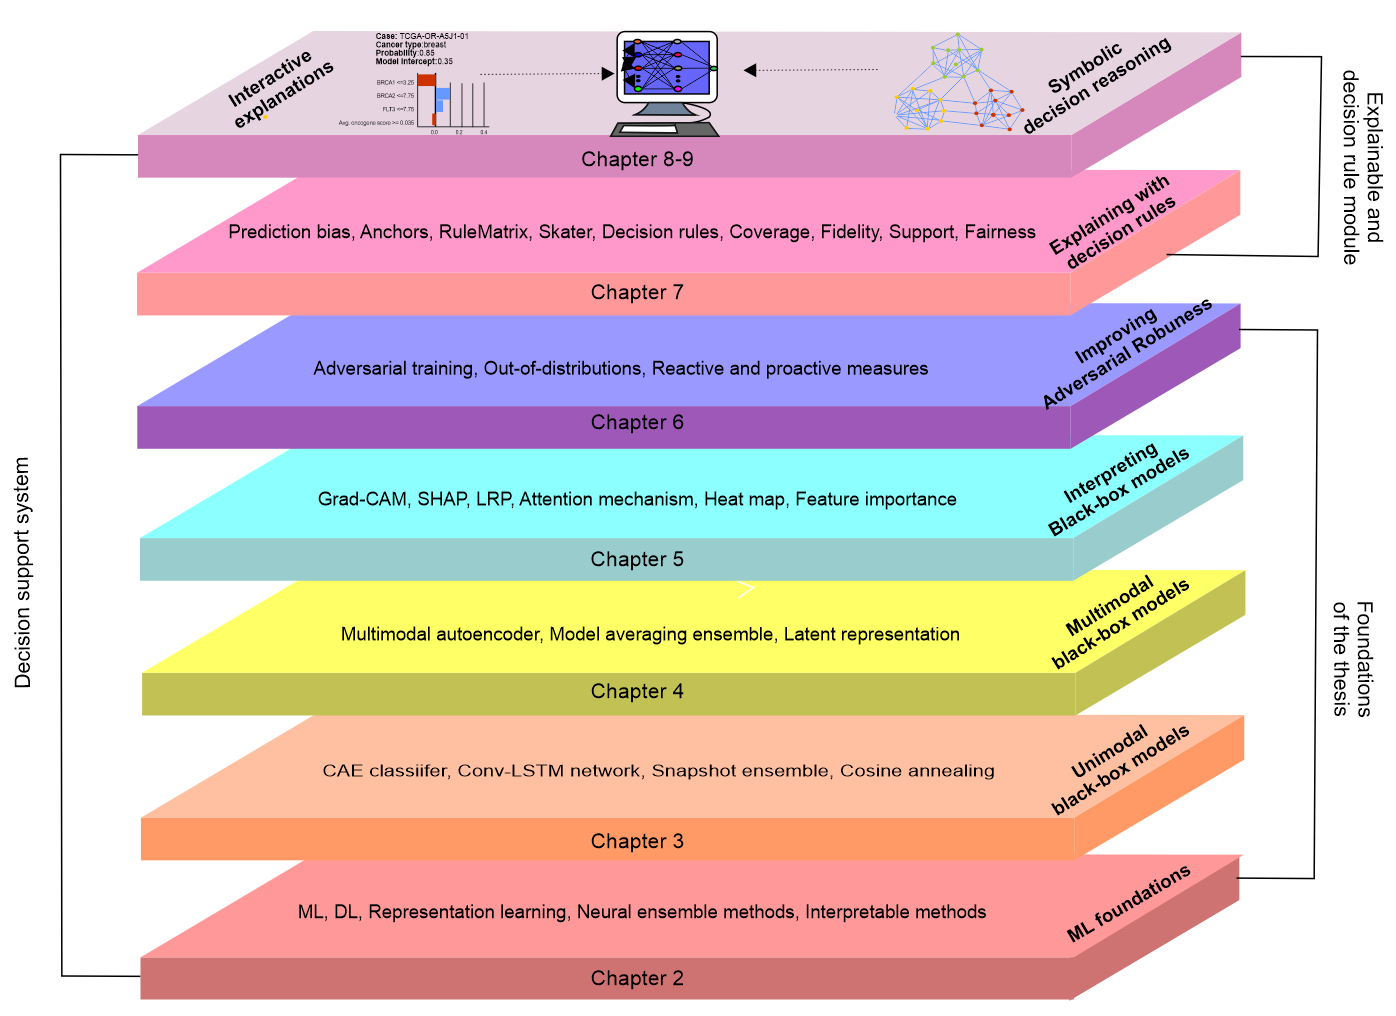
\includegraphics[width=0.9\linewidth,height=115mm]{images/chapter_outline.png}
		\caption{A bottom-up layout of the thesis, outlining the chapters}
        \label{fig:chapter_organization}
\end{figure*}

\section{Thesis Outline} \label{structure}
The rest of the thesis is structured into ten chapters. 
%The brief overview of each chapter is as followed: 
\Cref{chapter:preli} covers the foundations and concepts that will be used in the subsequent chapters. In \cref{chapter:uni_modality}, we develop predictive model based on single modality towards finding the association between CNV data and cancer, followed by the cancer type prediction task. In \cref{chapter:multiodality}, we extend the single modality based predictive model to multimodality-based cancer typing method by employing a multimodal neural network, but with a focus on breast cancer. In \cref{chapter:xai}, we employ two different approaches to open the `black box' uni/multimodal models towards making explainable predictions of cancer types based on different genomics data. Besides, we identify significant biomarkers and computed feature importance in terms of mean absolute impact to rank top genes across all the cancer types. In \cref{chapter:robustness}, we apply different types of adversarial attacks on our models, including image content moderation, numeric data moderation, and out-of-distribution, followed by assessing the robustness against these scenarios. 

\hspace*{3.5mm} In \cref{chapter:xai_rules}, we generate decision rules by combining model predictions and interpretations. Additionally, we identify  misclassified instances~(i.e., initial prediction by the model). In \cref{chapter:nsr}, we apply symbolic reasoning to provide diagnosis reasoning based on a domain-specific ontology; where, a reasoner decides whether a biological entity~(based on biomarkers and their attributes) is of correct types based on the ontological reasoning. The reasoner also help validate the findings and decision rules in order to deduce human-understandable decision rules. In \cref{chapter:fairness}, we improve the trustworthy of the diagnosis by combining model interpretations, decision rules, and decision reasoning. In \cref{chapter:end}, we provide explanations and points out the relevance of the study, highlights its limitations, and discusses future works before concluding the dissertation. 

